%
%	Begrifflichkeiten
%

\pagebreak
\section{NIS2}

\onehalfspacing

\subsection{The Network and Information Security Directive}

\subsection{Center for Internet Security}

\subsubsection{CIS Controls}

\subsubsection{CIS Benchmarks}

\subsubsection{Social Media and Loneliness}

According to a recent study conducted by the American Psychological Association, social distancing over an extended period can increase loneliness and significantly affect people's health.\footnote{See \textit{Luchetti, M. (2020)}: The trajectory of loneliness in response to COVID-19. \cite{apaLoneliness}}

\subsection{Rancher}

\begin{figure}[H]
\centering
\caption {Rancher Dashboard}
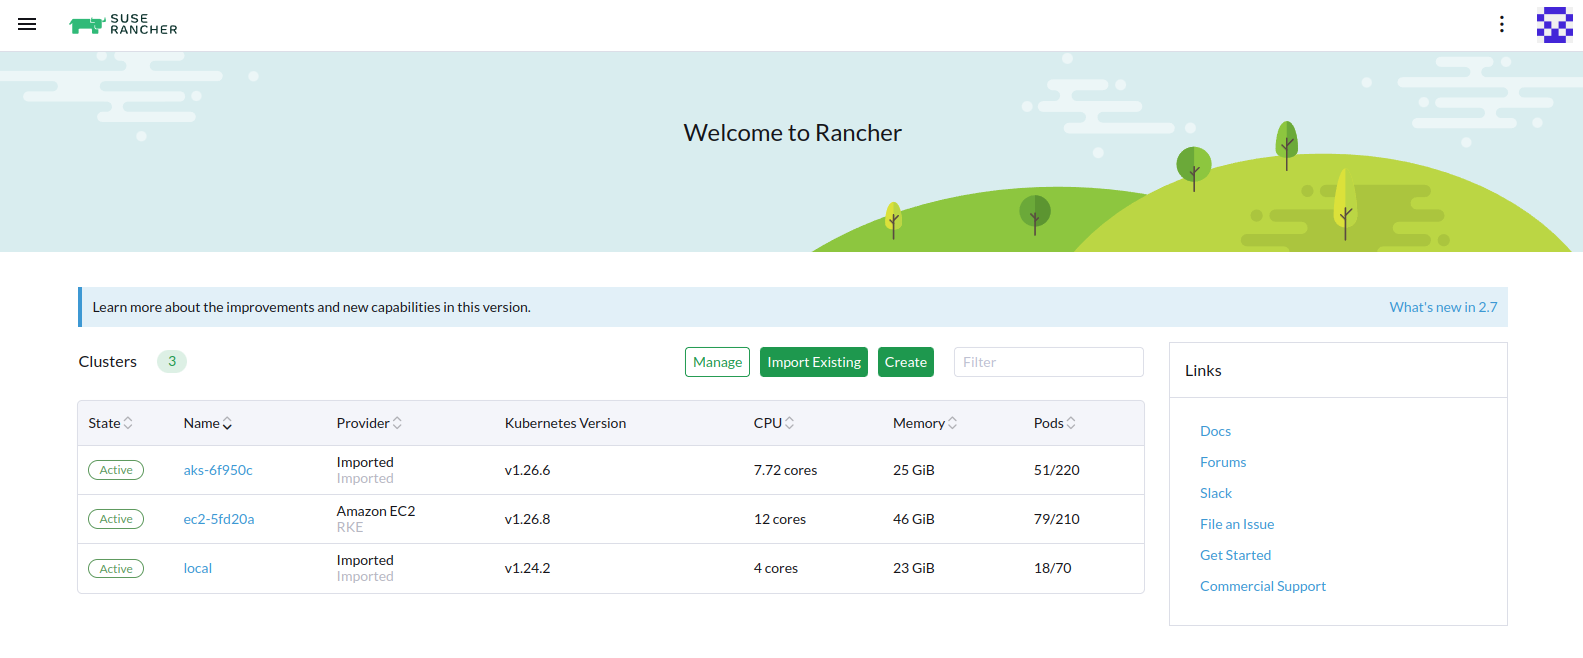
\includegraphics[width=\linewidth]{images/rancher-dashboard.png}
\label{fig:rancherDashboard}
\end{figure}

\subsubsection{CIS Benchmarks}

\subsubsection{CIS Benchmarks Installation}

\begin{lstlisting}[caption=Installing CIS, frame=single, basicstyle=\ttfamily]
# CIS Benchmarks
resource "rancher2_app_v2" "cisbench_fom" {
  lifecycle {
    ignore_changes = all
  }
  cluster_id = rancher2_cluster.cluster_fom.id
  name = "rancher-cis-benchmark"
  namespace = "cis-operator-system"
  project_id = data.rancher2_project.system.id
  repo_name = "rancher-charts"
  chart_name = "rancher-cis-benchmark"
  chart_version = var.cischart
}

\end{lstlisting}

\subsubsection{CIS Benchmark Reports}

\begin{itemize}
 \item wp-admin: The information in this table is only affecting me as the author of the paper, so no change is necessary
 \item wp-comments: I'll remove anything that could potentially identify the person commenting as well as all meta information and an empty column.
 \item wp-pages: The table has no personally identifiable information
 \item wp-search: The table has no personally identifiable information
 \item wp-visit: The table has no personally identifiable information
 \item wp-visitor: I'll remove all information, including IP Address, that could potentially identify the visitor
\end{itemize}
